\documentclass{beamer}
\usepackage[utf8]{inputenc}
\usepackage[T1]{fontenc}
\usepackage[francais]{babel} 
\usepackage{lmodern}
\usepackage{hyperref}
\usepackage{tikz}

\usetikzlibrary{trees,shapes.geometric,arrows,decorations.pathmorphing,backgrounds,fit,positioning,shapes.symbols,chains	}
 \tikzset{
    %Define standard arrow tip
    >=stealth',
    %Define style for boxes
    punkt/.style={
           rectangle, dashed,
           rounded corners,
           draw=black, very thin,
           minimum height=2em,
           minimum width = 2cm,
           text centered},
    square/.style={
           rectangle,
           draw=black, thick,
           minimum height=.5cm,
           minimum width = 1cm,
           text centered},
    data/.style={
           rectangle,
           draw=black, thick,
           minimum height= 2cm,
           minimum width = 2cm,
           text centered},
    % Define arrow style
    pil/.style={
           ->,
           thick,
           shorten <=1pt,
           shorten >=1pt,},
    asym/.style={
           <->,
           thin,
           shorten <=1pt,
           shorten >=1pt,
           red!100},
    sym/.style={
           <->,
           thin,
           shorten <=1pt,
           shorten >=1pt,
           blue!100}
}
\usepackage{pgfplots}
\usepackage{eurosym}
\usepackage{rotating}
\usepackage{array}
\usepackage{tikz-uml}
\usepackage{color, colortbl}
\usetheme{Antibes}
\usecolortheme{beaver}
\setbeamertemplate{sections/subsections in toc}[square]
\setbeamertemplate{blocks}[square]%

\author{Charles Ango - Ismaël Kabore - Julien Legras - Yves Nouafo - Jean-Baptiste Souchal}
\title{Projet annuel - Chat sécurisé}
\titlegraphic{
\includegraphics[height=3em]{logo_univ.png}}
\institute{Master 1 Sécurité des Systèmes Informatiques}

\date{18/01/2013}

\begin{document}
{
\setbeamertemplate{headline}[default] 
\begin{frame}
  \titlepage
\end{frame}
}

\frame{
\frametitle{Sommaire}
\tableofcontents
}

\section{Présentation du projet}
\frame{
\frametitle{Présentation du projet}
\begin{block}{Sujet proposé par Maglie Bardet}
	Réaliser un logiciel de messagerie instantanée sécurisée : client et serveur.\\
	S'inspirer des fonctionnalités d'IRC (Internet Relay Chat).
	Fonctionnalités demandées :
	\begin{itemize}
		\item gestion de la création et la suppression d'un compte sécurisé;
		\item création par un utilisateur d'une salle de discussion pour un groupe de personnes ;
		\item ajout/suppression d'un utilisateur autorisé dans une salle;
		\item assurance de confidentialités, d'intégrité et d'authentification sur les messages échangés;
		\item non-répudiation des messages.
	\end{itemize}
\end{block}
}

\section{Digramme de cas d'utilisation}
\frame[allowframebreaks=1.0]{
\frametitle{Digramme de cas d'utilisation}
\begin{tikzpicture}[scale=0.7, every node/.style={scale=0.7}]
\umlactor{User}
\umlactor[x=14, y=4]{AC}

\umlusecase[x=3, y=2, width=3cm]{Création compte sécurisé}
\umlusecase[x=10, y=4, width=3cm]{Suppression compte sécurisé}
\umlusecase[x=3, y=-1]{Rejoindre Server}

\umlusecase[x=7, y=1]{Quitter Server}
\umlusecase[x=10, width=3cm]{Envoi message privé}
\umlusecase[x=10, y=-2, width=3cm]{Envoi message au salon général}
\umlusecase[x=7, y=-3]{Déconnexion}

\umltrans{User}{usecase-1}
\umltrans{AC}{usecase-2}
\umltrans{User}{usecase-3}

\umlinclude{usecase-1}{usecase-2}

\umlextend{usecase-4}{usecase-3}
\umlextend{usecase-5}{usecase-3}
\umlextend{usecase-6}{usecase-3}
\umlextend{usecase-7}{usecase-3}
\end{tikzpicture}

\framebreak
\begin{center}
\begin{tikzpicture}[scale=0.4, every node/.style={scale=0.4}]
\umlactor[y=16]{User S}
\umlactor[y=5]{Admin}

\umlusecase[x=4, y=16, width=2.5cm]{Rejoindre Server S} % 8
\umlusecase[x=6, y=20]{Quitter Server S}				% 9
\umlusecase[x=9, y=19]{Suppression compte}				% 10
\umlusecase[x=10, y=18]{Déconnexion}                    % 11
\umlusecase[x=10, y=16, width=3cm]{Envoi message privé sécurisé}    % 12
\umlusecase[x=9, y=14, width=3cm]{Envoi message sur salon général}			% 13
\umlusecase[x=7.5, y=12, width=3cm]{Rejoindre salon privé} % 14
\umlusecase[x=14, y=12, width=2.5cm]{Quitter salon privé} % 15
\umlusecase[x=2.5, y=12, width=2.5cm]{Demande rejoindre salon}					% 16
\umlusecase[x=5, y=10]{Créer salon privé}				% 17
\umlusecase[x=14, y=10]{Invitation User S}				% 18
\umlusecase[x=12,y=7,width=3cm]{Envoi de message dans salon} % 19
\umlusecase[x=10,y=5,width=3cm]{Fermeture du salon privé} % 20
\umlusecase[x=6,y=8.5]{Exclure User S}						%21

\umltrans{Admin}{User S}
\umltrans{User S}{usecase-8}
\umltrans{Admin}{usecase-18}
\umltrans{Admin}{usecase-19}
\umltrans{Admin}{usecase-20}
\umltrans{Admin}{usecase-21}

\umlextend{usecase-9}{usecase-8}
\umlextend{usecase-10}{usecase-8}
\umlextend{usecase-11}{usecase-8}
\umlextend{usecase-12}{usecase-8}
\umlextend{usecase-13}{usecase-8}
\umlextend{usecase-14}{usecase-8}
\umlextend{usecase-16}{usecase-8}
\umlextend{usecase-17}{usecase-8}

\umlextend{usecase-15}{usecase-14}
\umlextend{usecase-19}{usecase-14}

\umlinclude{usecase-18}{usecase-14}
\umlinclude{Admin}{usecase-17}

\end{tikzpicture}
\end{center}
}


\section{Architecture du logiciel}
\subsection{Schéma global et entités}
\frame{
\frametitle{Schéma global et entités}
\begin{columns}
    \begin{column}{.5\linewidth}
      \begin{center}
		\begin{tikzpicture}[node distance=-.01cm,font=\tiny]
		\node[square, text width=1cm, fill=white!100] (appclient) at (0,0) {Application client};
		\node[square, text width=1.5cm, fill=white!100] (modclientsec) at (2.5,0) {Module client sécurisé};
		\begin{pgfonlayer}{background} 
		\node[punkt, fit=(appclient)(modclientsec), fill=blue!20] (groupclient) {};
		\end{pgfonlayer}
		
		\node[square, text width=1cm, fill=white!100] (PKI) at (1.4,-1.5) {PKI};
		\node[square, text width=1cm, fill=white!100] (serveur) at (0,-2.5) {Serveur};
		\node[square, text width=1.5cm, fill=white!100] (serveurs) at (2.5,-2.5) {Serveur sécurisé};
		\begin{pgfonlayer}{background} 
		\node[punkt, fit=(PKI)(serveur)(serveurs), fill=green!20] (groupserveur) {};
		\end{pgfonlayer}

		\node[text width=.7cm] (imgbd1) at (0,-4) {
\includegraphics[height=3em]{computer-database.png}};
		\node[square, text width=.5cm, below=of imgbd1, fill=white!100] (bd1){BDD};
		\node[text width=.7cm] (imgfichiers) at (1.4,-4) {
\includegraphics[height=3em]{system-file-manager.png}};
		\node[square, text width=1cm, below=of imgfichiers, fill=white!100] (fichiers){Fichiers};
		\node[text width=.7cm] (imgbd2) at (2.8,-4) {
\includegraphics[height=3em]{computer-database.png}};
		\node[square, text width=.5cm, below=of imgbd2, fill=white!100] (bd2){BDD};

		\begin{pgfonlayer}{background} 
		\node[punkt, fit=(imgbd1) (bd1) (imgbd2) (bd2) (imgfichiers) (fichiers), fill=orange!20] (stock) {};
		\end{pgfonlayer}


		\draw (appclient.east) edge[<->] (modclientsec.west);
		\draw (appclient.south) edge[<->] (serveur.north);
		\draw (appclient.south east) edge[<->] (PKI.north);
		\draw (modclientsec.south) edge[<->] (serveurs.north);
		
		\draw (serveur.south) edge[<->] (imgbd1.north);
		\draw (serveurs.south) edge[<->] (imgbd2.north);
		\draw (PKI.south) edge[<->] (imgfichiers.north);
		\draw (PKI.south east) edge[<->] (serveurs.north);
		
		\draw (PKI.west) edge[->, loop left = 90] (PKI.west);

		\end{tikzpicture}
  	  \end{center}
    \end{column}
    \begin{column}{.5\linewidth}
      API client :
      \begin{itemize}
      	\item sécurisé
      	\item non-sécurisé
      \end{itemize}
      
      Serveurs :
      \begin{itemize}
      	\item sécurisé
      	\item non-sécurisé
      	\item PKI
      \end{itemize}
      
      Données :
      \begin{itemize}
      	\item BDD serveur sécurisé
      	\item BDD serveur non-sécurisé
      	\item liste certifications/ révocations
      \end{itemize}
    \end{column}
  \end{columns}
}

\subsection{Fonctionnement}
\frame{
\frametitle{Fonctionnement}
\begin{center}
\begin{tikzpicture}[node distance=-.01cm,font=\footnotesize]
\node[square, text width=1.5cm] (clientsec1) at (0,0) {Client sécurisé};
\node[square, right=of clientsec1, text width=1.5cm] (clientchat1) at (2,0) {Client de chat};
\node[] (client1) at (1.5, -1) {Client 1};
\node[punkt, fit=(clientsec1)(clientchat1)(client1)] (group1) {};

\node[square, text width=1.5cm] (serveurchat) at (4.5,1.1) {Serveur de chat};
\node[square, text width=1.5cm] (serveurs) at (4.5,2.5) {Serveur sécurisé};

\node[square, text width=2cm] (ac) at (4.5,4.3) {Autorité de certification};


\node[square, text width=1.5cm] (clientchat2) at (6,0) {Client de chat};
\node[square, text width=1.5cm, right=of clientchat2 ] (clientsec2) at (8,0) {Client sécurisé};

\node[] (client2) at (7.5, -1) {Client 2};
\node[punkt, fit=(clientsec2)(clientchat2)(client2)] (group2) {};


\draw (clientsec1.east) edge[sym] node[above, align = center] {chiffré} (clientchat1.west);
\draw (clientsec2.west) edge[sym] node[above, align = center] {chiffré} (clientchat2.east);

\draw (clientchat1.north) edge[<->, bend left=20] (serveurchat.west);
\draw (clientchat2.north) edge[<->, bend right=20] (serveurchat.east);

\draw (clientsec1.north) edge[asym, bend left=30] node[above, align = center, rotate=45] {chiffré} (ac.west);
\draw (clientsec2.north) edge[asym, bend right=30] node[above, align = center, rotate=-45] {chiffré} (ac.east);

\draw (clientsec1.north) edge[asym, bend left=30] node[above, align = center, rotate=30] {chiffré} (serveurs.west);
\draw (clientsec2.north) edge[asym, bend right=30] node[above, align = center, rotate=-30] {chiffré} (serveurs.east);

\draw (ac.south) edge[<->] (serveurs.north);

\node[below=of group1] (legende) {Légende : \color{blue}$\leftrightarrow$ symétrique \color{red}$\leftrightarrow$ asymétrique};

\end{tikzpicture}
\end{center}
}

\subsection{Détails techniques}
\frame{
\frametitle{Détails techniques}
\begin{block}{Langages et bibliothèques}
\begin{itemize}
\item C $\rightarrow$ client et serveur
\item Vala $\rightarrow$ interface du client
\item GTK+ 3 $\rightarrow$ interface du client
\end{itemize}
\end{block}

\begin{block}{Sécurité}
\begin{itemize}
\item OpenSSL $\rightarrow$ implémentation Open Source de SSL et TLS
\item TinyCA vs EJBCA $\rightarrow$ EJBCA
\end{itemize}
\end{block}
}

\section{Organisation}
\frame[allowframebreaks=1.0]{
\frametitle{Organisation}
\begin{itemize}
        \item méthode agile
        \item découpage en sprints
        \item chaque sprint est basé sur une fonctionnalité
        \item fin de sprint $\rightarrow$ livraison d'un produit partiel fonctionnel
\end{itemize}
\begin{center}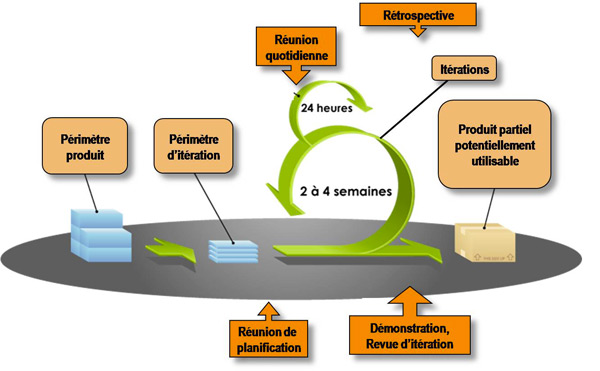
\includegraphics[height=12em]{scrum-agiles.jpg}\end{center}
\framebreak

Participation active du client :
\begin{itemize}
        \item sur les fonctionnalités de chaque sprint
        \item le test du livrable à chaque fin de sprint
\end{itemize}


Trois piliers:
\begin{itemize}
        \item transparence
        \item inspection
        \item adaptation
\end{itemize}

\framebreak
Les acteurs:
\begin{itemize}
        \item client
        \item scrum master
        \item développeurs
\end{itemize}

Adapté a notre projet:
\begin{itemize}
        \item chaque fonctionnalité est relativement courte
        \item 3 fonctionnalités principales :
        \begin{itemize}
                \item Client / Serveur (publics)
                \item PKI
                \item Client / Serveur (sécurisés)
        \end{itemize}
\end{itemize}                
}

\section{Planning de développement}
\frame[allowframebreaks=1.0]{
\frametitle{Planning de développement}
\begin{block}{Sprint 1 : Implémentation du client et du serveur simples}
\begin{itemize}
\item Serveur simple : la gestion des connexions à la base de données, des salons et la transmission de messages aux destinataires.
\item Client simple : la connexion et la déconnexion au serveur, l'envoi et la réception d'un message au serveur et l'interfaçage.
\end{itemize}
\end{block}

\framebreak

\begin{block}{Sprint 2 : Implémentation de la PKI et des échanges entre le client et la PKI}
\begin{itemize}
\item PKI : la certification de clef RSA, la vérification, l'envoi et le stockage des certificats.
\item Client : demande et de réception de certificat.
\end{itemize}
\end{block}

\framebreak
\begin{block}{Sprint 3 : Implémentation du client et du serveur sécurisés}
\begin{itemize}
\item Serveur sécurisé : la gestion des salons privés, des clefs de chiffrement symétrique, l'authentification lors de la connexion et l'enregistrement d'un nouvel utilisateur.
\item Client sécurisé : la gestion des clefs, le chiffrement/déchiffrement des messages, la création/suppression/administration de salon privé.
\end{itemize}
\end{block}
}

\section{Risques}
\frame{
\frametitle{Risques}
\tiny
\begin{center}
\begin{tabular}{|p{0.2cm}|p{2cm}|p{2cm}|l|l|l|c|}
\hline
\textbf{Réf.} & \textbf{Description} & \textbf{Facteurs} & \textbf{Type} & \textbf{Probabilité} & \textbf{Impact} & \textbf{Criticité} \\
\hline
R1&Utilisation de Git&Une seule personne sait l'utiliser&Tech&FORT&MAJEUR&20\\
\hline
R2&Apprentissage de Gtk, Vala&3 ont déjà fait du Vala, 1 du Gtk&Tech&MAJEUR&MAJEUR&15\\
\hline
R3&Apprentissage d'OpenSSL&Personne n'a déjà utilisé OpenSSL&Tech&FORT&MAJEUR&20\\
\hline
R4&Membre de l'équipe gravement malade&Environnement&RH&FAIBLE&MAJEUR&10\\
\hline
R5&Vol/Incident matériel&&RH&FAIBLE&CRITIQUE&12\\
\hline
R6&Utilisation d'une PKI (tinyca/EJBCA)&Faibles connaissances des PKI&Tech&MAJEUR&MAJEUR&15\\
\hline
R7 & Retard dans la livraison & Retard du développement d'une tâche bloquante & RH/Tech & MAJEUR & MAJEUR & 15\\
\hline
\end{tabular}
\end{center}
}

\end{document}